\documentclass[portrait]{a0poster}

\usepackage{aas_macros}
\usepackage{amsmath}
\usepackage{amssymb}
\usepackage{fontspec}
\usepackage{natbib}
\usepackage{graphicx}
\usepackage{xcolor}
\usepackage{lettrine}
\usepackage{flowfram}
\usepackage{tikz}
\usetikzlibrary{calc,matrix,shapes.geometric,shapes.misc,shapes.symbols}

% Macros
\newcommand{\EM}[1]{\ensuremath{\textsc{\textrm{em}}_#1}}
\newcommand{\GW}{\ensuremath{\textsc{\textrm{gw}}}}
\newcommand{\dropcap}[2]{\lettrine{\fontspec{Copse}#1}{\textnormal{#2}}}

% Adjust section style
\makeatletter
\renewcommand{\section}{\@startsection
{section}%                   % the name
{1}%                         % the level
{0mm}%                       % the indent
{-\baselineskip}%            % the before skip
{0.5\baselineskip}%          % the after skip
{\fontspec{Marvel Bold}\Huge}} % the style
\makeatother

% Adjust journal abbreviation style for AAS journal macros
\makeatletter
\let\jnl@style=\sf
\makeatother

% Adjust default font
\setsansfont[Mapping=tex-text]{Corbel}
\renewcommand{\familydefault}{\sfdefault}

% Adjust style for emphasized text
\renewcommand{\emph}[1]{{\bfseries\itshape#1}}

% Expand space between lines
\linespread{1.2}

% Increase paragraph indentation
\setlength{\parindent}{4em}

% Flow frames
\newstaticframe{\textwidth}{\textheight}{0.4\textwidth}{0.4\textheight}[watermark]
\newstaticframe{\textwidth}{0.3\textheight}{0\textwidth}{0.5\textheight}[title-drawing]
\newstaticframe{0.32\textwidth}{0.15\textheight}{0.34\textwidth}{0\textheight}[efficiency_distance]
\newstaticframe{0.32\textwidth}{0.15\textheight}{0.68\textwidth}{0\textheight}[efficiency_histogram]
\newstaticframe{0.32\textwidth}{0.15\textheight}{0.68\textwidth}{0.55\textheight}[convergence]
\newstaticframe{0.66\textwidth}{0.025\textheight}{0.34\textwidth}{0.75\textheight}[ligosmile]
\newstaticframe{0.32\textwidth}{0.32\textwidth}{0\textwidth}{0\textheight}[healpix-dots]
\newflowframe{0.32\textwidth}{0.025\textheight}{0.34\textwidth}{0.35\textheight}
\newflowframe{0.32\textwidth}{0.2\textheight}{0.34\textwidth}{0.15\textheight}
\newflowframe{0.32\textwidth}{0.2\textheight}{0.68\textwidth}{0.15\textheight}
\newflowframe{0.32\textwidth}{\textheight}{0\textwidth}{0\textheight}
\newstaticframe{0.32\textwidth}{0.5\textheight}{0.34\textwidth}{0.5\textheight}[flowchart]


\begin{document}

\begin{staticcontents*}{watermark}
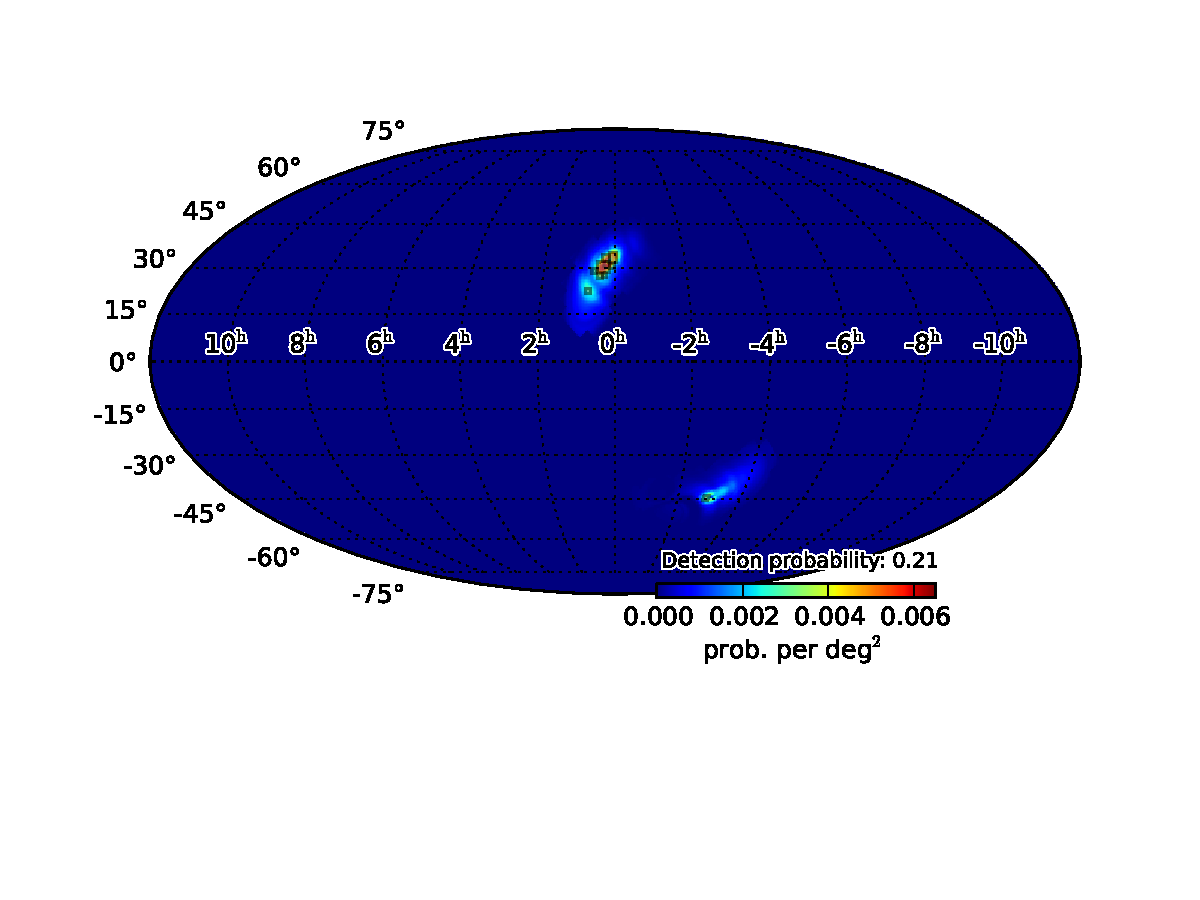
\includegraphics[scale=2]{example-no-interference}
\end{staticcontents*}

\begin{staticcontents*}{title-drawing}

\includegraphics[width=\textwidth,clip=true,trim=0cm 5cm 0cm 0cm]{title-drawing.pdf}
\end{staticcontents*}

\begin{staticcontents*}{efficiency_distance}
\includegraphics[width=\textwidth]{../efficiency_distance}
\end{staticcontents*}

\begin{staticcontents*}{efficiency_histogram}
\includegraphics[width=\textwidth]{../efficiency_histogram}
\end{staticcontents*}

\begin{staticcontents*}{convergence}
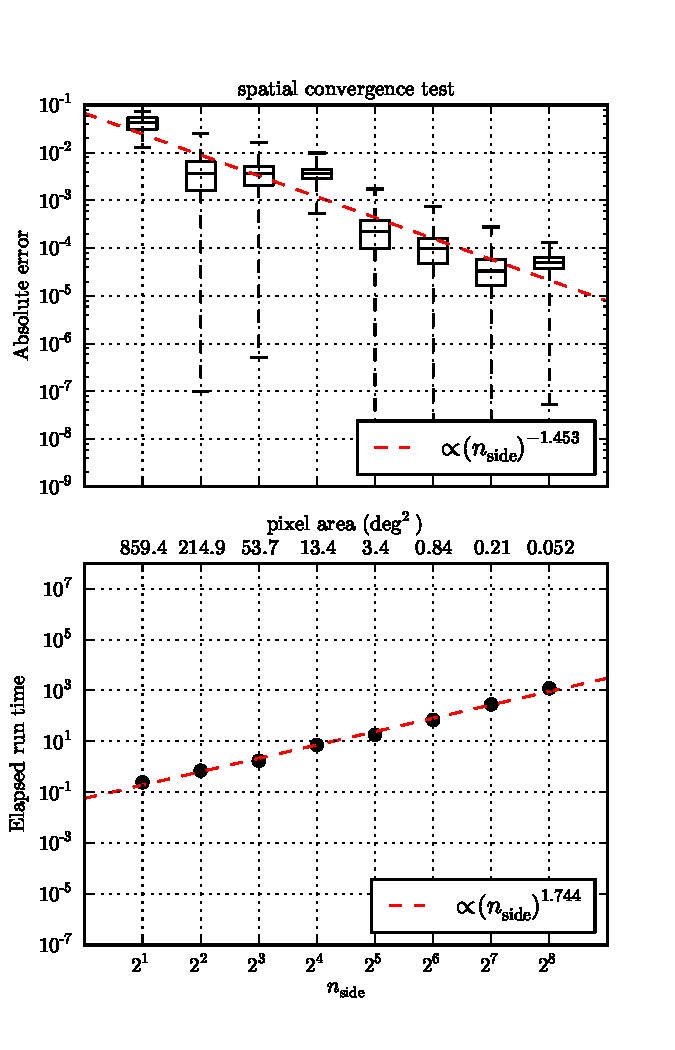
\includegraphics[width=0.5\textwidth]{spatial}
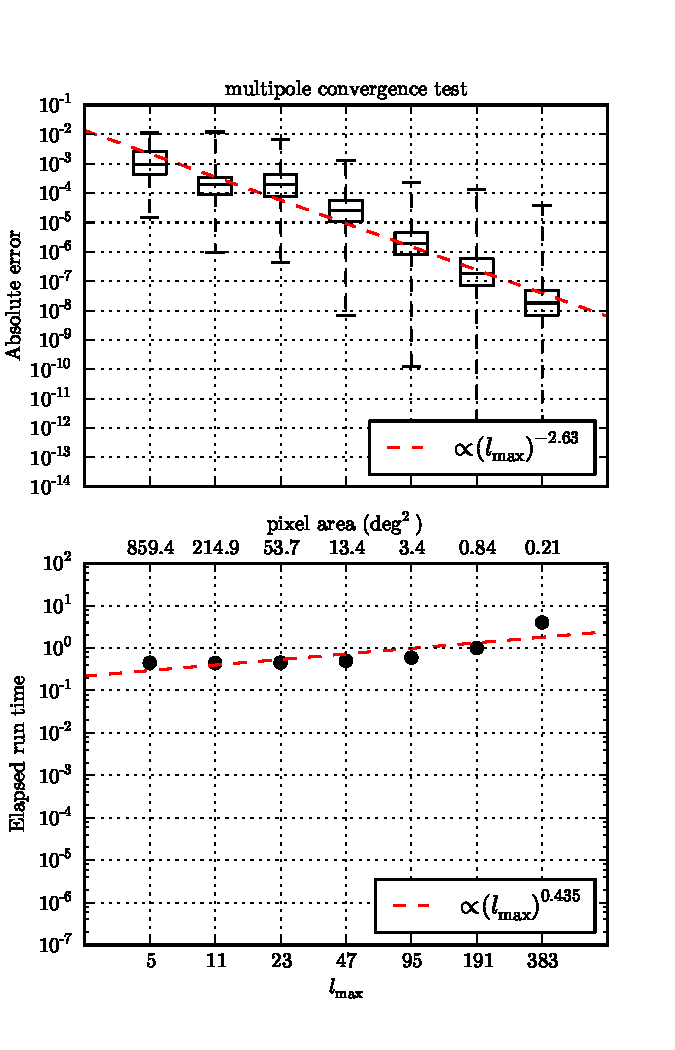
\includegraphics[width=0.5\textwidth]{multipole}
\end{staticcontents*}

\begin{staticcontents*}{healpix-dots}
\large\centering
figure 6d of~\citet{healpix}\\\vspace{5mm}
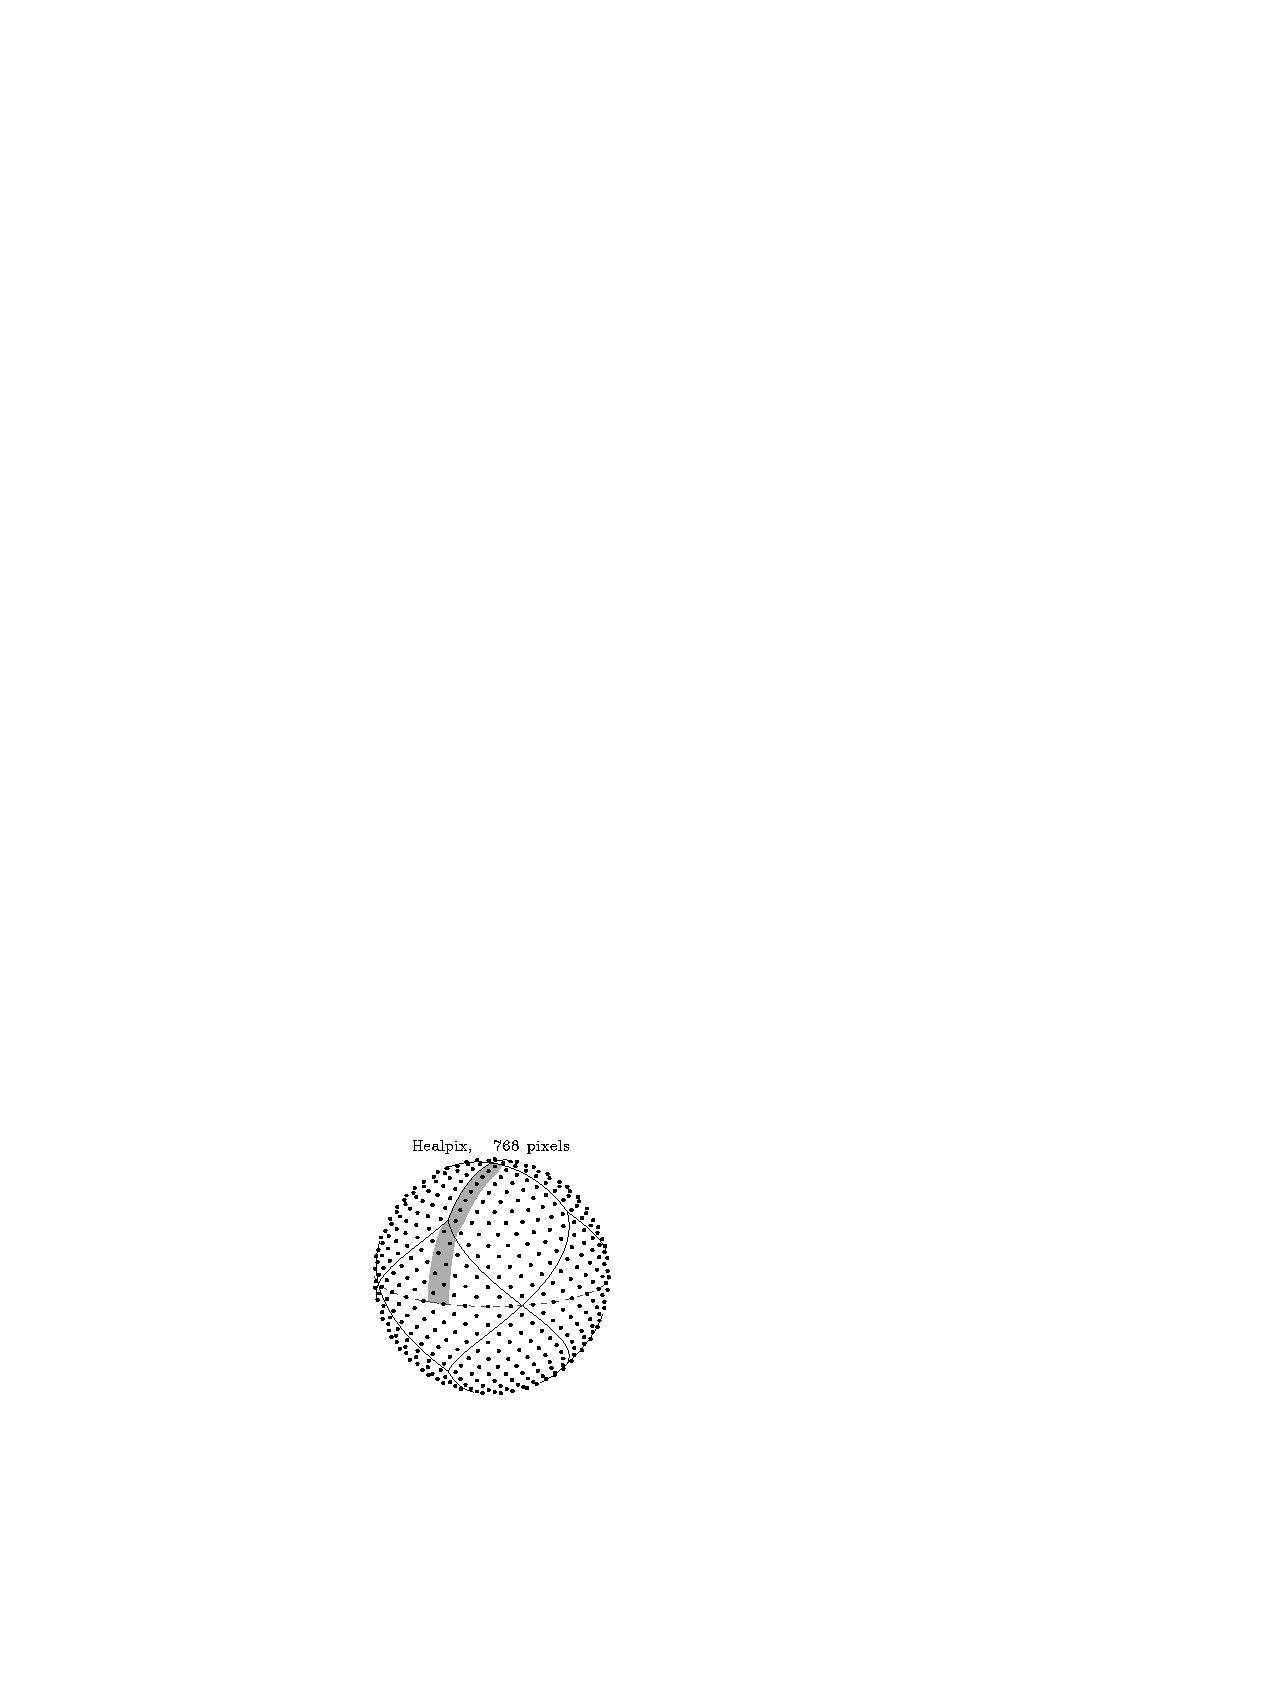
\includegraphics[width=\textwidth]{healpix-dots}
\end{staticcontents*}

\begin{staticcontents*}{ligosmile}
\begin{tabular}{ccccc}
\begin{minipage}[c]{0.3\textwidth}
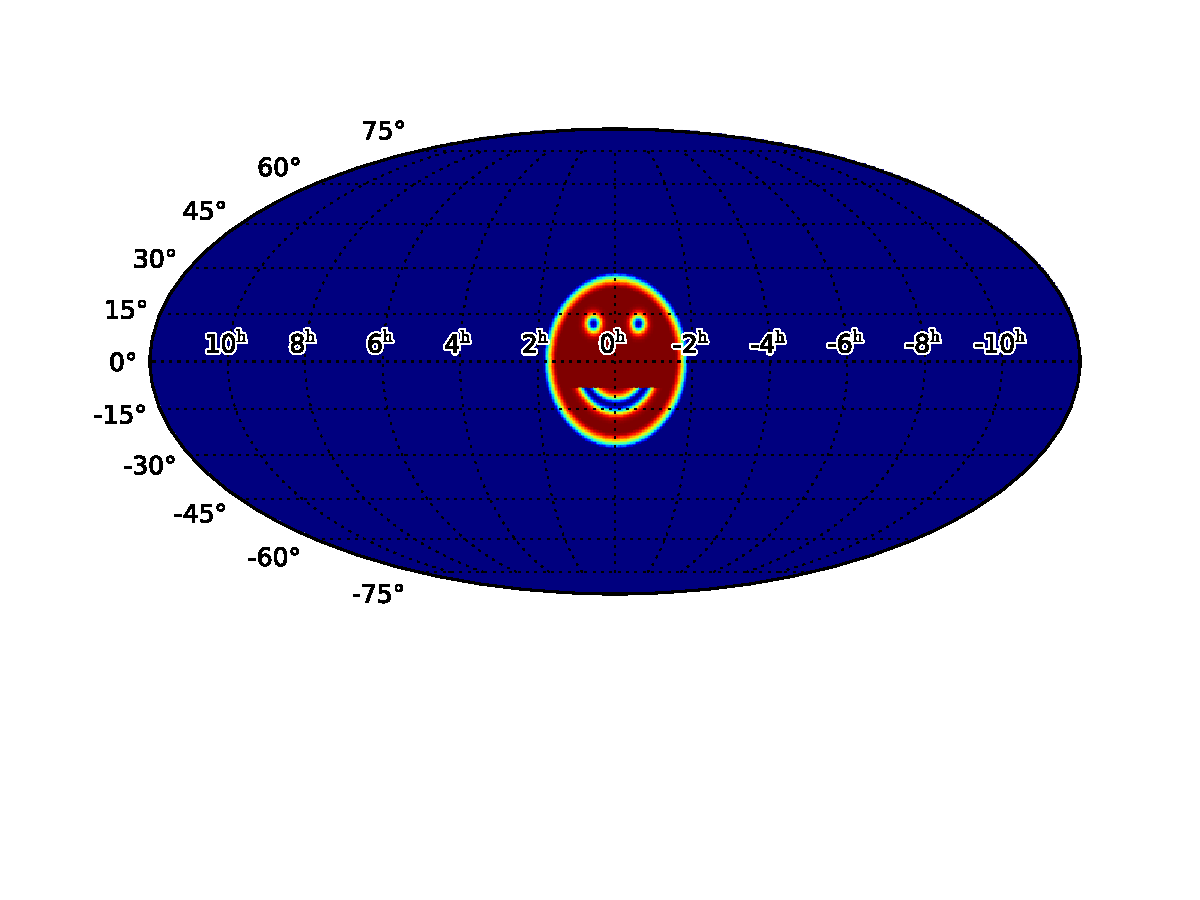
\includegraphics[width=\textwidth]{smile}
\end{minipage} &
{\Huge$\star$} &
\begin{minipage}[c]{0.3\textwidth}
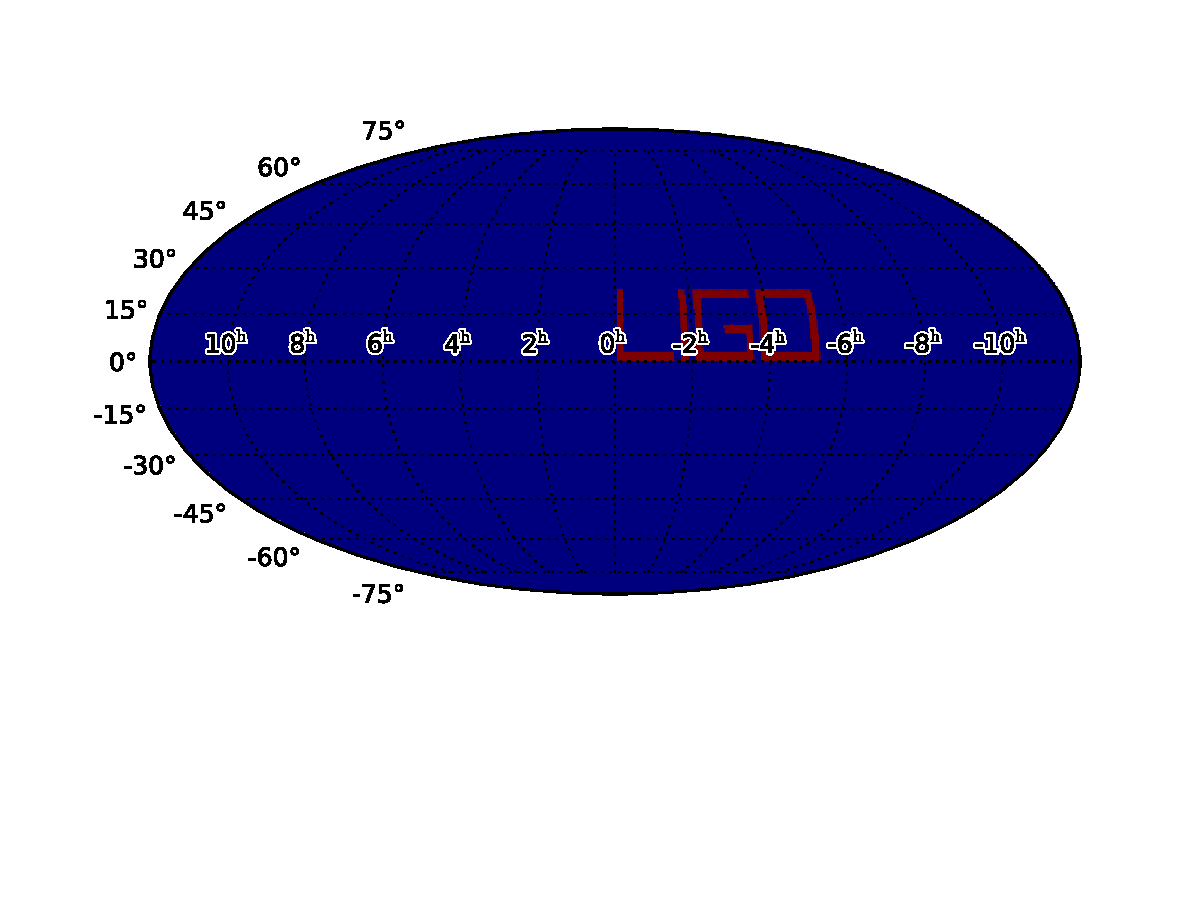
\includegraphics[width=\textwidth]{ligo}
\end{minipage} &
{\Huge$=$} &
\begin{minipage}[c]{0.3\textwidth}
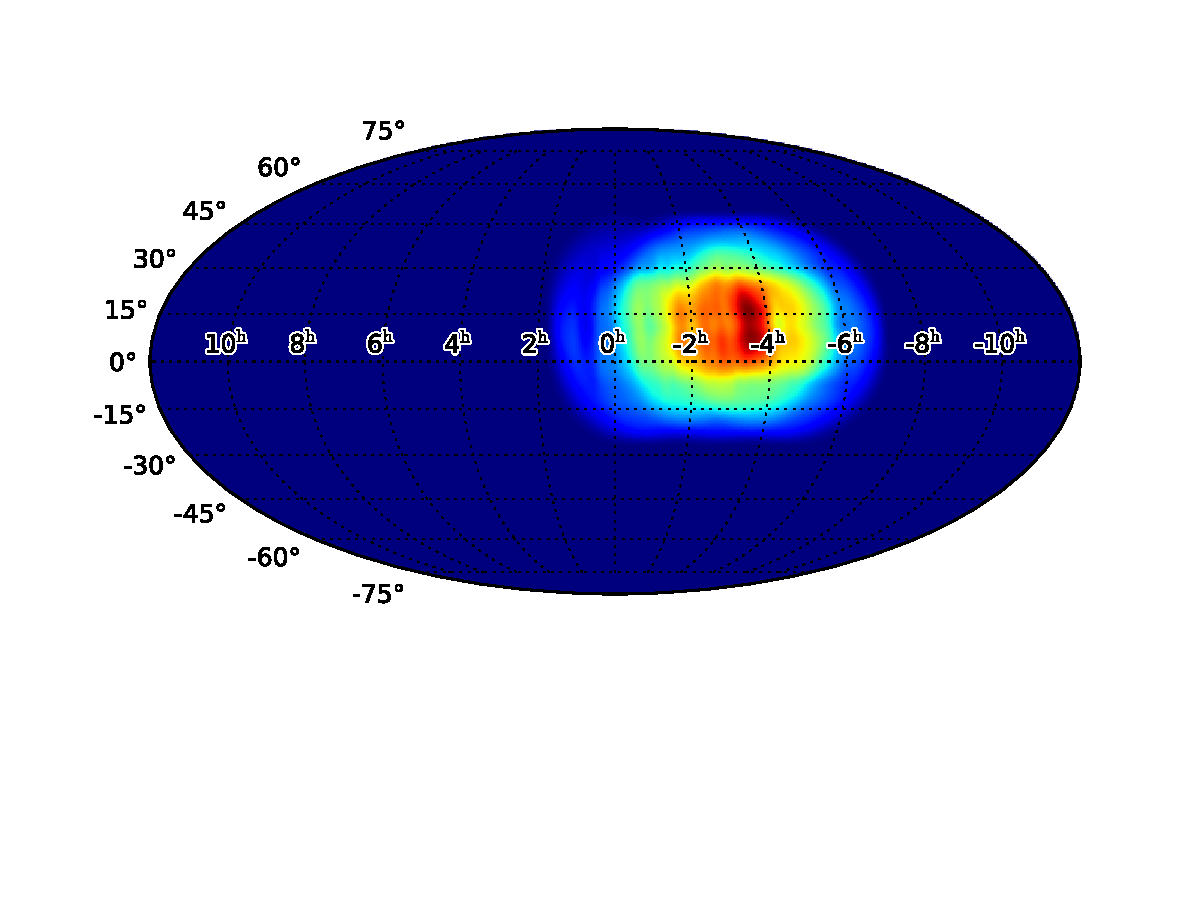
\includegraphics[width=\textwidth]{ligosmile}
\end{minipage} \\
{\fontspec{Marvel Bold}\huge Field of view} &
&
{\fontspec{Marvel Bold}\huge GW sky map} &
&
{\fontspec{Marvel Bold}\huge Cross-correlation}
\end{tabular}
\end{staticcontents*}

\begin{staticcontents*}{flowchart}
\pgfdeclarelayer{background layer}
\pgfdeclarelayer{foreground layer}
\pgfsetlayers{background layer,foreground layer}
\begin{tikzpicture}
	\begin{pgfonlayer}{foreground layer}
	\matrix (m) [
		matrix of nodes,
		row sep=2cm,
		every node/.style={fill=white, inner sep=0.75cm, anchor=center, align=center},
		every path/.style={line width=4pt}
	] {
		\node[draw, shape=rounded rectangle, text width=6cm] (1) {Begin}; \\
		\node[draw, shape=rectangle, text width=6cm] (2) {Read next telescope's FOV}; \\
		\node[draw, shape=rectangle, text width=10cm] (3) {Mask out parts of sky that are in daytime or twilight}; \\
		\node[draw, shape=rectangle, text width=6cm] (4) {Convolve FOV with skymap}; \\
		\node[draw, shape=rectangle, text width=6cm] (5) {Locate maximum}; & \node[draw, shape=starburst, random starburst=12, starburst point height=1.5cm] (55) {to telescope}; \\
		\node[draw, shape=rectangle, text width=6cm] (6) {Mask out FOV from skymap}; \\
		\node[draw, shape=diamond, aspect=2, text width=6cm] (7) {Any telescopes left?}; \\
		\node[draw, shape=rounded rectangle] (8) {Done}; \\
	};
	\end{pgfonlayer}
	\begin{pgfonlayer}{background layer}
	\draw[line width=4pt, ->] (1) -- (2);
	\draw[line width=4pt, ->] (2) -- (3);
	\draw[line width=4pt, ->] (3) -- (4);
	\draw[line width=4pt, ->] (4) -- (5);
	\draw[line width=4pt, ->] (5) -- (6);
	\draw[line width=4pt, ->] (6) -- (7);
	\draw[line width=4pt, line cap=rect, ->] (7) -- (8) node[very near start, right] {no};
	\draw[line width=4pt, ->] (5) -- (55);
	\draw[line width=4pt, line cap=rect] (7) -| ($(55.south)+(-2cm,-0.5cm)$) node[at start, above] {yes};
	\draw[line width=4pt, ->] ($(55.north)+(-2cm,0.5cm)$) |- (2);
	\end{pgfonlayer}
\end{tikzpicture}
\end{staticcontents*}

\section*{Background}

\framebreak

\dropcap{P}{lanning} telescope pointings for followup of gravitational wave (GW) events is a challenging optimization problem.  Probability maps conditioned on GW observations (GW sky maps) are multimodal and dispersed over 4π.

A telescope’s field of view (FOV) may have gaps between CCDs, dead CCDs, or vignetted or clipped regions.  Any of these complications make it harder to decide on the “best” place to point a telescope.

We realized that if we phrased the single telescope problem as a cross-correlation of the telescope’s FOV and the GW sky map, we could attack it with HEALPix --- the workhorse of CMB maps --- and spherical harmonic analysis.

Our summer student (A. Speranza) implemented the fast convolution of~\citet{Wandelt:2001p13439} and used it to compute the probability of imaging an EM counterpart.  As we expected, the harmonic analysis algorithm was much faster than the spatial algorithm.

What surprised us was that coordinating all of the observations by maximizing the probability of imaging the source conditioned on all of the telescopes’ pointings \emph{doubled} the number of detectable sources as compared to deciding each telescope’s configuration in isolation.

\framebreak

Our key results are the two figures below.  At left is the fraction of injected signals that we would have imaged with one pointing of each telescope at the time of the trigger as a function of luminosity distance.  Solid lines represent observing plans that account for interference from the Sun and Earth.  Dashed lines represent observing plans in which these considerations are neglected.

We tested three different planning algorithms:

\paragraph{\color{red}noncooperative}
Each telescope is independently pointed where it is most likely to observe an EM counterpart.

\paragraph{\color{green!50!black}greedy sorted}
Suppose that we have chosen pointings for telescopes 1, 2, $\dots$, $i$.  The pointing of telescope $i+1$ is chosen to maximize the probability of detection, subject to telescopes 1, 2, $\dots$, $i$, remaining fixed.

\paragraph{\color{blue}anneal}
Uses simulated annealing to the probability of imaging the source by varying the configurations of all of the telescopes simultaneously.

\framebreak

\section*{Single telescope case}

\dropcap{S}{ky maps} are posterior distributions of source location $\omega$ given all GW observations \GW.  The GW sky map is
%
$$
	s(\omega) \triangleq p(\omega | \GW).
$$
%
Let $\EM{i}$ denote the event of observing an optical transient with telescope $i$.  Let $\gamma_i$ represent the pointing of telescope $i$.  The probability of observing an EM counterpart in telescope $i$ given its pointing $\gamma_i$ is
%
$$
	b_i(\gamma_i^{-1} \omega) \triangleq p(\EM{i} | \gamma_i, \omega).
$$
%
Now, marginalizing over the unknown source location, this becomes
%
\begin{equation}
	\label{eq:single-telescope-integral}
	p_i \triangleq p (\EM{i} | \gamma_i, \GW) = \int s(\omega) b_i(\gamma_i^{-1} \omega) \, \mathrm{d}\Omega.
\end{equation}
%
The optimal pointing of a single telescope (ignoring sun and horizon interference) is
%
$$
	\gamma_i^* \triangleq \arg \max_{\gamma_i} p(\EM{i} | \gamma_i, \GW).
$$

\section*{Numerical implementation}

\dropcap{E}{quation}~(\ref{eq:single-telescope-integral}) is strongly reminiscent of a cross-correlation integral with the kernel $b_i (\gamma_i^{-1} \omega)$.  For functions defined on the real number line, the convolution theorem and the fast Fourier transform (FFT) provide a fast convolution algorithm.  \citet{Driscoll1994202}, \citet{Wandelt:2001p13439}, and many others have provided analogous fast convolution algorithms on $S^2$.

We used HEALPix to write two convolution algorithms:

\paragraph{spatial} uses nearest neighbor interpolation of the rotated kernel to approximate the integral in spherical polar coordinates.

\paragraph{multipole} uses the fast convolution algorithm of~\citet{Wandelt:2001p13439}.  It entails a spherical harmonic transform of both the sky map $s(\omega)$ and the FOV $b(\omega)$, a weighted inner product of the spherical harmonic coefficients, and finally a 2D inverse FFT to return to polar coordinates.\\

We tested the rate of convergence and run time of both algorithms.  (For the multipole algorithm, we tested for self-convergence.)  For a resolution of $\approx$~0.05~deg$^\mathsf{2}$, the spatial algorithm took about 1000~s while the multipole algorithm took only about 4~s.

Both algorithms are parallelized with OpenMP, so both will be even faster on multicore machines (e.g. cluster head nodes).

\section*{Multiple telescope case}

\dropcap{F}{or} multiple telescopes, the figure of merit is the probability of imaging the source with at least one telescope:
$$
	p_{\geqslant 1} \equiv \sum_i p_i - \sum_{i \neq j} p_{ij} + \sum_{i \neq j \neq k} p_{ijk} - \cdots
$$
This is \emph{not} the same as the probability of imaging the source with telescope 1, or telescope 2, or telescope 3 \dots :
$$
	p_{1 \textrm{ or } 2 \textrm{ or } 3 \textrm{ or } \dots} = p_1 \, p_2 \, p_3 \dots \neq p_{\geqslant 1}
$$

\bibliographystyle{apj}
\bibliography{../proposal,../telescope,../telescope_list}

\section*{Acknowledgements}

LIGO was constructed by the California Institute of Technology and Massachusetts Institute of Technology with funding from the National Science Foundation and operates under cooperative agreement PHY-0107417.  This research is supported by the National Science Foundation through a Graduate Research Fellowship to LS.  This poster has LIGO Document Number LIGO-G1100983-v1.

\end{document}
